\documentclass{kththesis}

\usepackage{blindtext} % This is just to get some nonsense text in this template, can be safely removed

\usepackage{csquotes} % Recommended by biblatex
\usepackage[style=numeric,sorting=none,backend=biber]{biblatex}
\addbibresource{references.bib} % The file containing our references, in BibTeX format

\usepackage{pgfplotstable,filecontents}
\pgfplotsset{compat=1.9}% supress warning
\usepackage{booktabs,colortbl}

\title{This is the English title}
\alttitle{Detta är den svenska översättningen av titeln}
\author{Vilmer Jonsson \\ Tor Strimbold}
\supervisor{Kevin Smith}
\examiner{Pawel Herman} 
\programme{Bachelor's Degree in Computer Science}
\school{School of Electrical Engineering and Computer Science}
\date{\today}

% Uncomment the next line to include cover generated at https://intra.kth.se/kth-cover?l=en
\kthcover{kth-cover.pdf} % Cover page background file, placeholder for now


\begin{document}

% Frontmatter includes the titlepage, abstracts and table-of-contents
\frontmatter

\titlepage

\begin{abstract}
  English abstract goes here.

  \blindtext
\end{abstract}


\begin{otherlanguage}{swedish}
  \begin{abstract}
    abstract på svenska.
  \end{abstract}
\end{otherlanguage}


\tableofcontents


% Mainmatter is where the actual contents of the thesis goes
\mainmatter


% TODO: Fix the references
\chapter{Introduction}
The frequency of malignant melanoma has in the last decade been on the rise with approximately 60 000 people being diagnosed with the disease yearly \parencite{sverige-hudcancer}.
A similar trend has been observed in the United States where the frequency of people diagnosed with the disease has doubled yearly from 1982-2011 \parencite{aad-skin-cancer}.

% TODO: Fix the references, could not find the source in Drive
Skin cancer, although common, has a survival rate of up to 95\% if discovered at an early stage. %(källa)
This fact makes the diagnosis of malignant melanoma an essential part of the treatment of the disease. In the light of diagnosis, machine learning has become a subject of interest in many medical fields, dermatology included. Multiple studies have been conducted to evaluate the potential of the algorithms’ accuracy and applicability through so-called computer aided diagnostics (CAD). Concerning malignant melanoma, some studies have reached an accuracy of up to 90\% which competes with the experts in the field. %(källa). 

The accuracy of machine learning algorithms is however heavily reliant on the feature extraction methods used, where relevant features in an image are extracted and then used in the classification of the skin lesion. An effective feature extraction in turn relies on determining which features to use. Which is the subject of feature selection where different features are compared in terms of their effect on the diagnostic accuracy. It has been shown that effective feature selection make classifiers more effective, accurate and cost-effective. \parencite{KarabulutEsraMahsereci2012Acso}

\section{Research Question}
In our thesis we will study the effect of two different feature selection methods upon 169 features and using 4 different machine learning models. We aim to answer:
\begin{enumerate}
    \item Which features and combinations of features are the most important in terms of classification accuracy?
    \item Is there a difference between different models concerning which features are most effective?
    \item Are some feature selection methods more efficient in creating better accuracy than others? Which one uses the fewest number of features?
  
\end{enumerate}

\section{Approach}

To study the proposed research questions both forward and backwards selection will be performed. To further widen the base for comparison four different machine learning models will be used: support vector machine, random forest, k-nearest neighbors and a one-layered neural network. These models are widely used in the research of automatic skin lesion diagnosis which makes them relevant to study. % Källa
Furthermore, two selection methods will be used, namely sequential forwards selection and sequential backwards selection. 

The features to be used in the feature selection are of two classes: handcrafted and automatically generated features. The handcrafted features are based on the clinical practice through the ABCD method where a skin lesion is classified based on its asymmetry, border irregularity, color and diameter. The ABCD method is widely used when diagnosing skin lesions using ML due to its effectiveness and simplicity to implement. \parencite{JAIN2015735}
Thus making it relevant to the study. For the automatically generated features, SIFT was chosen as the feature. % It is relevant because … (Is it really necessary to explain why SIFT is relevant here?)

% A little bit outdated.
Lastly the base of comparison will be widened by the use of two different datasets will be used in the study, namely the HAM10000 and ISIC dataset. 

A comparison between the classifiers, where first no selection is done and then between the two selection methods, will be conducted. The result from this will then highlight whether different features have different impact on the efficiency and accuracy of machine learning algorithms. Furthermore, it will show if certain features are to be preferred in the context of different machine learning models. Lastly, it will show if there is any difference between the handcrafted and automatically generated features.

\section{Scope}

The study is limited by the number of features, selection methods and models being used.

Firstly the models are limited by the fact that they consist of only machine learning. An extension of the study could include a deep learning model such as a convoluted neural network.

Secondly, the study is limited by the feature selection methods being used where only feature selection by wrapper methods are used through the sequential backward and forward selection.

Lastly, the study is limited by the features which the selection is based in three different ways. Firstly, not all combinations of the features will be examined since this would require too many computations. Secondly, the different aspects of the ABCD method can be extracted in a plethora of different ways, which leaves room for further studies. Thirdly, the features are only of two types of classes, other classes such as bag-of-features will not be used.


\chapter{Background}

\section{Skin Cancer}

% https://www.ncbi.nlm.nih.gov/pmc/articles/PMC8705277/ bra artikel


% Lite upprepning från introduktionen ksk, men fortfarande bra att ha med
During the last  decades the frequency of malignant melanoma in Sweden has been on the rise and the trend does not seem to be going down. Yearly, approximately 60 000 persons are diagnosed with skin cancer and around 500 die from the disease. \parencite{sverige-hudcancer}

Likewise in the United States, skin cancer is the most common type of cancer to the degree that every fifth american will develop the disease at some time during their lives. The rates of melanoma have on a general trend increased, nearly doubling between 1982-2011. On some levels the rates have decreased, as in for people that are under 30. \parencite{aad-skin-cancer}

Malignant melanoma is a type of skin cancer that is the result of melano\-cyte cells in the skin starting to grow uncontrollably.
Although melanoma is a less common type of skin cancer, it is at the same time more prone to spreading to other parts of the body therefore making it more dangerous. \parencite{aad-skin-cancer}

Melanoma skin cancer has five different stages, stage 0-5, where in stage 0 the cancer is contained within the top layer of the skin while in the final stage the cancer has spread to other parts of the body \parencite{cancerresearchuk-melanoma}.
According to UK researchers the survival rate of patients diagnosed with melanoma differs greatly depending on when during the four different stages the diagnosis is made \parencite{cancerresearchuk-survival}.
Where if the cancer is detected in the first stage the survival rate is almost 100\%, however if the diagnosis is done in a later stage the survival rate drops to 30\%, although the statistic does not take into account the age of the patients. \parencite{cancerresearchuk-survival}

Recently artificial intelligence (AI) and machine learning (ML) has made great strides within dermatology in areas such as melanoma detection and classification. In one study, a machine learning algorithm was compared against experts, where the ML system outperformed the experts. \parencite{8030303}

% \subsection{Computer Aided Diagonstics} Might be a good idea to have a section about CAD, but I'm not sure if it's necessary.

\section{Machine Learning}

% https://ietresearch.onlinelibrary.wiley.com/doi/full/10.1049/iet-ipr.2015.0385?sid=vendor%3Adatabase (abcd)

Machine learning (ML) is a field of computer science focusing on automated and intelligent data analysis. A ML algorithm is fed problems and answers whereupon the system tries to predict the answer. Based on the response the algorithm then makes adjustments to better give the correct answers. \parencite{das2021machine}

In the case of skin cancer detection, an ML algorithm would receive images with a ground truth for each image, meaning either the skin lesion is malignant or benign. The algorithm would then try to correctly decide if the lesion is cancerogenous thereafter the correct answer would be revealed and the algorithm makes corrections based on whether or not it was successful in the diagnosis.

An ML algorithm consists of four main steps: 1) pre-processing, 2) segmentation, 3) feature extraction and 4) classification. All of the named steps are described below.

\subsection{Pre-processing}

The main goal with pre-processing an image is to improve the quality of the picture. Improvement can be made in many ways but generally the methods can be sorted into either artifact removal or image enhancement \parencite{8377976}.
Artifact removal entails removing misleading objects in the image such as hair pixels and air bubbles which can lead to incorrect segmentation and feature extraction. Image enhancement usually consists of contrast Pre-processing is an essential step in the process since the classification is vastly dependent on the image quality. \parencite{jaworek2016automatic}

\subsection{Segmentation}

In the segmentation phase the borders of the lesion are identified. This is done to be able to identify what in the image contains the lesion. Like the pre-processing, segmentation is vital for the classification and feature extraction since parameters such as the lesion’s border cannot be correctly evaluated if the segmentation is poorly executed. At the same time, the segmentation of skin lesions is one of the most challenging steps due mainly to four reasons. Firstly, most lesions do not have a stark contrast between the healthy and unhealthy skin. Secondly, the lesion’s border may be irregular which impedes the segmentation. Thirdly, the color variegation % (huh, typ skilland)
within the lesion can be vast where multiple colors are present at the same time. Finally, there may be artifacts such as hairs or lens flare present within the image which hinders the segmentation, this is however meant to be removed during the pre-processing. \parencite{jaworek2016automatic}

\subsection{Feature Extraction}

Clinical classification is done based on the characteristics of the lesion. Likewise, the features of the lesion need to be quantified in a way that a computer can understand to make a classification. This is the goal of feature extraction, to quantify the relevant characteristics of the lesion. Which features to consider relevant depends on the base of classification, the same holds for the way to extract the features.

\subsubsection{ABCD}

The ABCD-rule is a mimic of the way clinicians determine whether or not a skin lesion is malignant or not based on four features: asymmetry, border, colour and dermoscopic structures or diameter of the lesion. The higher the asymmetry of the lesion, in terms of either shape or colour, the more likely it is to be malign. The border aspect refers to whether the border of the lesion is irregular. The lesion is divided into eight slices and for each slice, if the border is irregular a point is awarded. Regarding the colour, the lesion is scanned for the occurrence of six colours (white, red, light brown, dark brown, blue-grey and black). For each colour a point is awarded. The “D” in ABCD can either be evaluated using the dermoscopic structure or the diameter of the lesion. The dermoscopic structure is evaluated based on the presence of five structures. For each structure a point is awarded, so the values range from zero to five. If instead the diameter is evaluated, all lesions with a diameter greater than 6 mm are considered malignant and given a value of five. \parencite{smaoui2013developed} \parencite{https://doi.org/10.1049/iet-ipr.2015.0385}

\subsubsection{Scale-invariant feature transform (SIFT)}

Scale-invariant feature transform (SIFT) is a popular method to extract key points out of an image. These key points are detected by an algorithm and given descriptors based on why the points were considered important. These descriptors can then be used in a classifier.

SIFT features are, as previously mentioned, used widely in the broader image analysis field. However, the research where the features are used to classify melanoma is quite limited.

\section{Classification}

The classification of the lesions based on the features extracted can be done through several machine learning algorithms. The ones used in this study are listed below.

\subsection{Support Vector Machine (SVM)}

Support vector machines (SVM) are common and effective ML algorithms first introduced in the 1990s. SVM is an extension of the support vector classifier, which in turn is an extension of the maximal margin classifier.

The maximal margin classifier aims to separate data into two classes using a hyperplane. The support vector classifier builds on the same principle, but is more adjusted to the case when the data is not easy to separate. The SVM enlarges the feature space of the data in order to be able to separate data in a non-linear fashion. \parencite{james2013introduction}

%% TODO: Fix references from here. The book above needs paging.
% Based on: book s.340-341, 344-345, 349-354

% One very good study with accuracy of 97.5\% <- det här är en bra studie för att få ut grejer om feature extraction också, snackar om något som heter hog features

% hej vilmer testa den här länken
% hej vilmer här är en till länk
% bok att hämta sen
% bok om alla algoritmer typ 

\subsection{Random Forest (RF)}

Random forest is a tree-based method. The model consists of several decision trees taking different factors into consideration. When classifying, all individual trees try to classify the data. Then, the class that most of the trees predicted is chosen as the final classification.

% book s. 319-321
% s. 319-321

\subsection{K-Nearest Neighbors (KNN)}

K-nearest-neighbors is another method for classifying. The ground principle is to find the nearest neighboring data points from the training set for all the test data points. In a similar fashion to random forest, it performs a majority voting and then chooses the most occurring class from neighbors as the final prediction.

% book  s.39-41
% Image on p. 40 in the book

\subsection{Neural Network (NN)}

% TODO: Fix this section
Neural networks are a type of machine learning algorithm that is inspired by the human brain. The network consists of several layers of neurons, where each neuron is connected to all neurons in the previous layer. The first layer is the input layer, where the data is fed into the network. The last layer is the output layer, where the final prediction is made. The layers in between are called hidden layers. The hidden layers are the ones that do the actual work of the network. The neurons in the hidden layers are connected to all neurons in the previous layer, and the output of each neuron is calculated by a function. The output of the neurons in the last hidden layer is then fed into the output layer, where the final prediction is made. \parencite{ibmWhatNeural}


% Neural network is a type of machine learning algorithm, inspired by the human brain, and consists of several connected layers of nodes. There are three types of layers, namely input, output and hidden layers. 
% beskriv hur en nod fungerar
% beskriv hur data går igenom alla noder
% Detta fixade co-pilot lol, men är väl versionen ovan som gäller?

\section{Feature selection}

% https://www.jmlr.org/papers/volume3/guyon03a/guyon03a.pdf
% ! Inte tillagd i referenslistan

Feature selection is a process where the different extracted features are ranked in order of importance for the results of the classification. Some features may be irrelevant and thus confusing for the model. The goal for feature selection may vary, but it is commonly used to find the most important features, features that harm the results and synergies between features. In short, reducing the number of features utilized, improves performance and accuracy. \parencite{chaganti2022thyroid}

In this study the greedy methods Sequential Backward Selection (SBS) and Sequential Forward Selection (SFS) will be used.

Sequential backward selection is a process that involves multiple iterations in which a feature is eliminated during each cycle. In the initial iteration, the feature that results in the worst performance, according to some metric, when removed is excluded from the set. The process is then repeated with the updated set of features. This process is continued until the desired number of features are left. \parencite{chaganti2022thyroid}

Forward selection shares the same underlying concept as backward selection, but instead begins with a smaller feature set and adds one feature during each iteration, resulting in an increased set of features rather than a reduced one.


\section{Related Works}

% TODO: Fix the references in this section. E.g. "Första" corresponds to a specific reference
% Note that "andra" were not used.

% ! I won't fix more of this now as it will be changed

The automatic classification of skin lesions as being either malignant or benign has been a subject of great interest and there is a plethora of publications investigating the manner. Hence, there are several studies focused around classifying lesions, using the feature set and ML models which this thesis aims to investigate. However, there is not such an abundant pool of studies which focus on feature selection methods and exploration of which types of features are the most important. 

\parencite{MustafaSuleiman2017Fsus} studied the minimal number of necessary features for effective and accurate skin lesion classification using a KNN-model.  The features that were studies were based on the geometric (A), color (C)  and boundary (B) aspects of the ABCD rule of melanoma.(\parencite{MustafaSuleiman2017Fsus}) A feature selection method which implemented the Sequential Backward Selection (SBS) was used. When all features (15 in total) were used, the average accuracy was around 78\%. The highest accuracy of 91\% was obtained when there were only 6, 8 and 9 features. Hence, \parencite{MustafaSuleiman2017Fsus} showed that an effective feature selection method both improves the accuracy of the classifier as well as the computation and storage cost. Though they did not highlight which of these features were abundant and which were important to include. Additionally they only limited the study to one type of ML model, namely the KNN. 

Tre studied the effect of feature selection using the NCA method with an M-SVM on three different data sets. Like \parencite{MustafaSuleiman2017Fsus} their method showed an increase in accuracy and runtime. However, as well as \parencite{MustafaSuleiman2017Fsus}, they did not investigate which features were the ones leading to the increased accuracy. Furthermore, only one classifier was used with the M-SVM and therefore no results were generated using some other type of classifier. 

Fyra used ECNA feature selection to gain succesful results. The highest accuracy reached was 94.73\% using a KNN and second best was using an SVM with and accuracy of 93.83\%. They however, used deep features instead of the hand crafted features which will be used in this study.


\chapter{Methods}

\section{Machine learning methods}

\subsection{Preprocessing}

For removing artifacts such as hairs, the DullRazor® software was used. The software is created by Tim Lee, Vincent Ng, RIchard Gallagher, Andrew Coldman and David Mclean and is used frequently for preprocessing of skin lesion images. The method removes the hairs in two steps: 1) using generalized grayscale morphological closing operations, it identifies the dark hair locations, 2) verifies the shape of the hair pixels as long and thin, thereafter it replaces the verified pixels by bilinear interpolation and lastly 3) smooths the replaced hair pixels. \parencite{dermwebDullRazor} % den här källan är ksk lite scuffed. Fanns en referens på själva sidan vi kanske borde ta istället.

% TODO: Download and insert the images from the google drive

\subsection{Segmentation}

The aim of this study was not to develop a new segmentation method, but rather to compare the effect of different feature selection methods on the accuracy of the classification. Therefore, the segmentation was done using open-source software published by [name] available on GitHub.

\subsection{Feature extraction}

As mentioned in the background, the two feature extraction methods used were ABCD and SIFT.

\subsubsection{ABCD} % morphological ?

The asymmetry and border features are calculated through the method proposed by \parencite{inproceedings} and the color features by \parencite{celebi2008automatic}. Both computations showed promising results reaching an accuracy of 82\% and 83\%. Furthermore, other morphological features are calculated using the scikit skimage measure package. The implementation is originally done in the way described in this Github repository \parencite{melanoma-classifier}.

% TODO: Dubbelkolla namn på library. Det är fel
To calculate the asymmetry and border features the measure library from sci-kit is used, with the \verb|get_region_props| function.
The color features are calculated using a numpy array to represent the image's RGB value.

% TODO: Lägg in hur man beräknar grejerna, eller ska det ens in?

% Hur de beräknas
% github repot

\subsubsection{SIFT}

The SIFT features are extracted using the OpenCV class SIFT which implements the algorithm by David G. Lowe. \parencite{sift-opencv} \parencite{lowe2004distinctive}.
After that...

% Vilket bibliotek
% opencv

\subsection{Classification}

All classifiers used in this study are from the Scikit-sklearn library which is a free-to-use library for machine learning in Python \parencite{scikit-learn-doc}.

% ! Nedanstående stämmer typ inte längre. Ska vi skriva något om parameter sweep? Vi gjorde ju lite.
Although all ML models’ parameters can be fine-tuned to optimize performance and run-time, the default parameters will be used since it is not the aim of the study to create an optimal implementation. The focus is instead on the feature selection’s effect on the performance of the classifiers.

% (källa ?)

\section{Dataset}

The dataset used in this study is a variant of the one produced by the ISIC Archive. The difference with the original one is that the one used only has two classes: Malignant and Benign. The dataset contains around 3400 images, each being 224x224 pixels. The dataset is balanced, which has positive effects on the classifiers accuracy. The larger, but unbalanced, HAM10000 dataset was also considered. However, during initial testing it was discovered that the balanced dataset resulted in a better accuracy. It was also easier to work with the balanced dataset, as it already only had two classes while HAM10000 has 7.

The dataset was downloaded and structured in order to have every image in the same folder. In order to store the ground truth information indicating whether a given image is malignant or benign, a one-dimensional array was created storing boolean values.

\section{Metrics}

\subsection{Accuracy}

Accuracy is a metric which is widely used and simple to calculate.  
It is calculated by dividing the total number of correctly classified images with the total number of images. 
It therefore measures the probability that the model will classify a given random image correctly. \parencite{takiddin2021artificial}

Accuracy was the metric used to determine the performance of the classifiers and the effect of the feature selection methods.


\section{Feature selection}

All feature selection methods used in the study originates from the \verb|Scikit-sklearn| library \verb|feature_selection|.

The manner in which the feature  selection was performed differs slightly due to the selection method employed. For the SFS, the feature set was initially empty. The method then adds all features, one at a time. For the SBS the feature set at first contained all features, whereupon features were removed one at a time, until the feature set consisted of only one feature. In each iteration, the accuracy and which features constituted the feature set were recorded. 
This process was repeated five times for every selection method and classifier. Hence, 40 tests were conducted in total.
% TODO: Write that we did the tests five times for each classifier and feature selection method

\section{Evaluation}

The method for evaluating the three different research questions are stated below.

\subsection{Is there a difference between different models concerning which features are most effective?}
Furthermore, since in every iteration of the selection methods, the included features were recorded, the features included in the feature set generating the optimal accuracy was determined. Onwards, this feature set will be referred to as the optimal feature set. 

Based on this statistic, the probability that a feature would be included in the optimal feature set, was calculated by dividing the number of times the feature was included in the optimal feature set with the number of tests performed. The features with the highest probability can therefore be seen as the most important.

\subsection{Which features and combinations of features are the most important in terms of classification accuracy?}
Based on the findings from the previous research question, the results were summarized to give insight on a more general level where the occurrences of each feature in the optimal feature set was divided by the total number of tests performed. This gives an insight into which features are most likely to constitute the optimal feature regardless of the classifier.

\subsection{Are some feature selection methods more efficient in creating better accuracy than others? Which one uses the fewest features?}
Since multiple tests were performed for every combination of classifier and selection method, it becomes possible to calculate the average accuracy for each number of features in the feature space. Hence the highest average accuracy and the expected number of features needed to achieve this accuracy can be determined. To determine which selection model is the most efficient, the difference between the original accuracy and the highest average accuracy using feature selection, was examined.


\chapter{Results}

Note that complete tables are found in the appendix. Only partial tables are presented in this chapter.

\section{Determining most important features}

% Could write more here.
Below is a table showing the features that were included in the optimal set the most and least amount of times. The features are sorted in descending order based on how many times they were included in the optimal feature set.

In the following table the thirteen most prominent, and twelve least prominent features are presented, overall. 

% Maybe put in a disclosure like this:
% It should be noted that some classifiers used more features than others, which explains why...


% Fråga inte hur detta funkar.
\begin{table}[h!]
  \begin{center}
    \caption{The most and least prominent features in all 40 tests.}
    \pgfplotstabletypeset[col sep=comma,
    string type,
    columns={Feature, Occurence(s), Probability},
    columns/Feature/.style={column name=Feature, column type={|l|}},
    columns/Occurence(s)/.style={column name=Occurence(s), column type={l|}},
    columns/Probability/.style={column name=Probability, column type={l|}},
    every head row/.style={before row=\hline, after row=\hline},
    every nth row={1}{before row=\hline},
    every nth row={13}{before row=\hline\hline}, % Cut in the table
    every last row/.style={after row=\hline},
    row predicate/.code={% display only the first 20 rows
    \ifnum#1>12\relax
    \ifnum#1<157\relax
    \pgfplotstableuserowfalse
    \fi
    \fi
    }
    ]{../big_data_new.csv}
  \end{center}
\end{table}
\newpage
In the table it is observable that two features stand out: number 151 and 160. These are both morphological features.% ABCD eller morphological? 

Feature 151 is called "Extent" and measure how many of the pixels in an image are within the lesion.
The extent feature was also the only feature that was included in the optimal feature set for all classifiers.

Feature 160 is a color feature that measures the red color of the image. It calculates the mean of the red color within the lesion and divides it by the mean of the red color in the parts of the image outside the lesion.

We can also see that there is a large spread, only two features are in the optimal feature set less than 25\% of the tests. Furthermore, the occurrences quickly deteriorate where the most prominent feature has 35 occurrences whereas the seventh most prominent feature only has 22 occurrences, which is a total difference of 13 occurrences. The downwards trend does however flatten out quickly as there are 52 features that have the occurrence of 20-17 occurrences. Lastly, the final span of 17 to 8 occurrences entails all the remaining features. 


Furthermore, we can also compare the two different sets of features, the handcrafted ABCD features and the automatically generated SIFT features.

% ! Fråga Kevin om detta är rätt
\begin{table}[h!]
  \caption{Average number of occurrences in optimal set for ABCD and SIFT features.}
  \pgfplotstabletypeset[ col sep=comma,
    string type,
    columns={Feature Type, Number of Features, Occurence(s), Representation},
    columns/Feature Type/.style={column name=Feature Type, column type={|l|}},
    columns/Number of Features/.style={column name=Feature count, column type={l|}},
    columns/Occurence(s)/.style={column name=Occurences, column type={l|}},
    columns/Representation/.style={column name=Average Occurences, column type={l|}},
    every head row/.style={before row=\hline, after row=\hline},
    every nth row={1}{before row=\hline},
    every last row/.style={after row=\hline}
  ]{../representation.csv}
\end{table}

From the results, it is observable that the SIFT features have more occurences overall than the morphological features. However, if the distribution between the two types is considered, the morphological features have a higher occurence rate per feature than the SIFT features, which can imply that the morphological features are more likely to be included in the optimal set.

\section{Determining important features for each classiifier}

To determine which features are important for different classifiers, the optimal feature set was examined in every test to see how many times a feature was included in the set. The results for each classifier is listed in the rubrics below.

\subsection{K-nearest neighbours}

Below are the two tables showing the most important features for KNN using SFS and SBS respectively. The features are sorted in descending order based on how many times they were included in the optimal feature set.

\begin{table}[h!]
  \begin{center}
    \caption{The features with at least 5 occurences in the 10 tests.}
    \pgfplotstabletypeset[col sep=comma,
    string type,
    columns={Feature, Occurence(s), Probability, Probability in SFS, Probability in SBS},
    columns/Feature/.style={column name=Feature, column type={|l|}},
    columns/Occurence(s)/.style={column name=Occurrence(s), column type={l|}},
    columns/Probability/.style={column name=Probability, column type={l|}},
    columns/Probability in SFS/.style={column name=Probability in SFS, column type={l|}},
    columns/Probability in SBS/.style={column name=Probability in SBS, column type={l|}},
    every head row/.style={before row=\hline, after row=\hline},
    every nth row={1}{before row=\hline},
    every last row/.style={after row=\hline},
    row predicate/.code={% display only the first 20 rows
    \ifnum#1>6\relax
      \pgfplotstableuserowfalse
    \fi
    }
    ]{../knn_total_probability.csv}
  \end{center}
\end{table}

The results show that the SFS preferred more features than the SBS counterpart. Furthermore, there is very little overlap between the preferred features when comparing the two methods. The only feature that has a probability of 80 percent or more is number 151, which were the most preferred across all classifiers. However, apart from the most common feature, the probability that a feature is included in the optimal set, is at most 50\%. Furthermore, this probability is shared by the following six features. Lastly, there was very little overlap in which features were included for the two methods.


% New page in order to not have the tables on the same page.
\newpage

\subsection{Neural Network}

\begin{table}[h!]
  \begin{center}
    \caption{The features with at least 9 occurrences in the 10 tests.}
    \pgfplotstabletypeset[col sep=comma,
    string type,
    columns={Feature, Occurence(s), Probability, Probability in SFS, Probability in SBS},
    columns/Feature/.style={column name=Feature, column type={|l|}},
    columns/Occurence(s)/.style={column name=Occurrence(s), column type={l|}},
    columns/Probability/.style={column name=Probability, column type={l|}},
    columns/Probability in SFS/.style={column name=Probability in SFS, column type={l|}},
    columns/Probability in SBS/.style={column name=Probability in SBS, column type={l|}},
    every head row/.style={before row=\hline, after row=\hline},
    every nth row={1}{before row=\hline},
    every last row/.style={after row=\hline},
    row predicate/.code={% display only the first 20 rows
    \ifnum#1>18\relax
      \pgfplotstableuserowfalse
    \fi
    }
    ]{../nn_total_probability.csv}
  \end{center}
\end{table}

The results show that the classifier included more features in the optimal set compared to other classifiers. The most prominent feature was 80, which is a SIFT feature which occurred in the optimal feature set in all tests. Furthermore, every feature was present in at least three of the tests. This can be seen in the appendix where the full table is presented.

\subsection{Random Forest}

\begin{table}[h!]
  \begin{center}
    \caption{The features with at least 8 occurences in the 10 tests.}
    \pgfplotstabletypeset[col sep=comma,
    string type,
    columns={Feature, Occurence(s), Probability, Probability in SFS, Probability in SBS},
    columns/Feature/.style={column name=Feature, column type={|l|}},
    columns/Occurence(s)/.style={column name=Occurence(s), column type={l|}},
    columns/Probability/.style={column name=Probability, column type={l|}},
    columns/Probability in SFS/.style={column name=Probability in SFS, column type={l|}},
    columns/Probability in SBS/.style={column name=Probability in SBS, column type={l|}},
    every head row/.style={before row=\hline, after row=\hline},
    every nth row={1}{before row=\hline},
    every last row/.style={after row=\hline},
    row predicate/.code={% display only the first 20 rows
    \ifnum#1>15\relax
      \pgfplotstableuserowfalse
    \fi
    }
    ]{../rf_total_probability.csv}
  \end{center}
\end{table}

Random forest, similar to Neural Network, included a lot of features in the tests. The most prominent features were 18, 94, 112, 131 and 100, which were SIFT features. They were present in the optimal feature set in all tests except one. In general the classifier seemed to prefer SIFT features where the highest ranked ABCD feature was 151 with a probability of 80\%.

\subsection{Support Vector Machine}

\begin{table}[h!]
  \begin{center}
    \caption{The features with at least 5 occurences in the 10 tests.}
    \pgfplotstabletypeset[col sep=comma,
    string type,
    columns={Feature, Occurence(s), Probability, Probability in SFS, Probability in SBS},
    columns/Feature/.style={column name=Feature, column type={|l|}},
    columns/Occurence(s)/.style={column name=Occurence(s), column type={l|}},
    columns/Probability/.style={column name=Probability, column type={l|}},
    columns/Probability in SFS/.style={column name=Probability in SFS, column type={l|}},
    columns/Probability in SBS/.style={column name=Probability in SBS, column type={l|}},
    every head row/.style={before row=\hline, after row=\hline},
    every nth row={1}{before row=\hline},
    every last row/.style={after row=\hline},
    row predicate/.code={% display only the first 20 rows
    \ifnum#1>10\relax
      \pgfplotstableuserowfalse
    \fi
    }
    ]{../svm_total_probability.csv}
  \end{center}
\end{table}

The SVM differs from the other classifiers, with a preference for morphological features. Consequently, all except number 151 were color features from the ABCD method. Furthermore, the occurences of features decrease quite rapidly where the seventh to eleventh most prominent features only have a probability of 50\% of being present in the optimal set. 


\section{Difference selection methods}

To examine eventual differences between the methods, two type of results were gathered. Firtly, the average number of features included in the optimal set. This was calculated by recording the number of features present in the optimal set for every test and then calculating the average of these. Secondly, the average difference in performance between the methods for every classifier. This was done by calculating the average accuracy of every iteration in the tests. The results are then plotted for every classifier. 

Following are the comparison between the two different selection methods. 

% TODO: Vill man plåga sig lite kan man försöka färga raderna.

\begin{table}[h!]
  \begin{center}
    \caption{The average number of features in the optimal set for the different classifiers and selection methods.}
    \pgfplotstabletypeset[col sep=comma,
    string type,
    columns={Classifier, Selection Method, Average Number of Features},
    columns/Classifier/.style={column name=Classifier, column type={|l|}},
    columns/Selection Method/.style={column name=Selection Method, column type={l|}},
    columns/Average Number of Features/.style={column name=Average Number of Features, column type={l|}},
    every head row/.style={before row=\hline, after row=\hline},
    every nth row={1}{before row=\hline},
    every last row/.style={after row=\hline},
    ]{../features_methods.csv}
  \end{center}
\end{table}

The results show that the SFS method used on average more features than the SBS method in all cases except for the Random Forest classifier. The biggest relative difference was in the case of the KNN classifier where the SFS method used more than twice the number of features than the SBS method. However, no test used all of the available features to achieve the highest accuracy.


% TODO: Hitta på bättre namn?
\subsection{Difference in performance between selection methods}

Following are the results related to the difference in performance between the two methods for every classifier.
\subsubsection{K-Nearest Neighbors}

\begin{figure}[h!]
  \begin{center}
    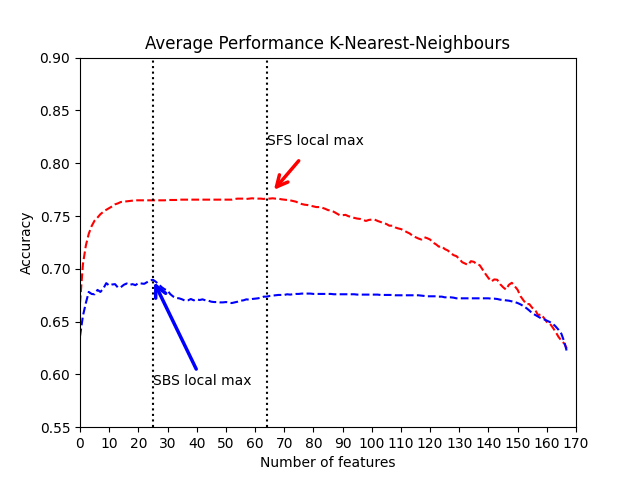
\includegraphics[scale=0.8]{./figures/Figure_2.png}
    \caption{Difference in performance for the KNN classifier}
  \end{center}
\end{figure}

The results show that the SFS achieved a greater increase in accuracy compared to the SBS method with an accuracy of about 78\% compared to 70\%. However, the SBS utilized less than half of the number of features compared to the SFS, where the former used around 35 features compared to the 65 features for the SFS.


\subsubsection{Neural Network}

\begin{figure}[h!]
  \begin{center}
    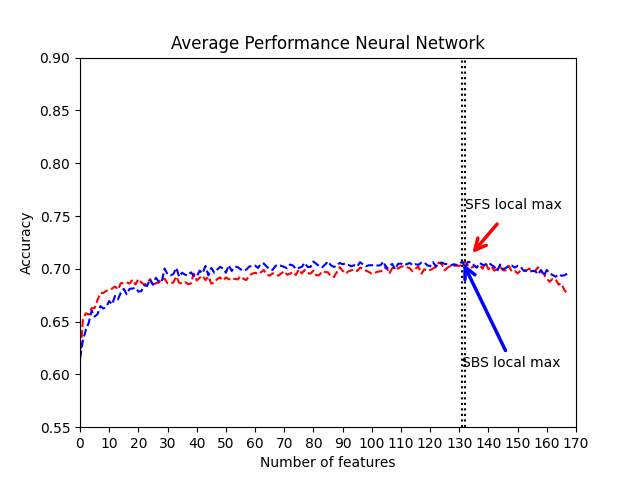
\includegraphics[scale=0.8]{./figures/Figure_1.png}
    \caption{Difference in performance for the NN classifier}
    \label{fig:nn}  % Used to add reference in text
  \end{center}
\end{figure}

Figure \ref{fig:nn} shows that the two methods had similar results for the neural network, both in terms of performance and number of features used. None of the methods resulted in any major gains in term of performance.

\subsubsection{Random Forest}

\begin{figure}[h!]
  \begin{center}
    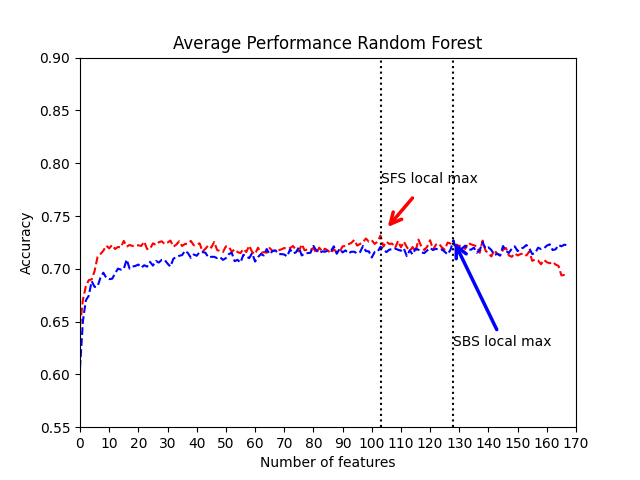
\includegraphics[scale=0.8]{./figures/Figure_4.png}
    \caption{Difference in performance for the RF classifier}
  \end{center}
\end{figure}

Similarly to the neural network, the difference between the two methods is not vast in terms of performance. The difference lies however within the number of features used where the SFS used fewer features than the SBS method. Furthermore, it is observable that there is minimal gain for the SFS method when using over 100 features compared to using between 30 and 10 features.

\newpage

\subsubsection{Support Vector Machine}

\begin{figure}[h!]
  \begin{center}
    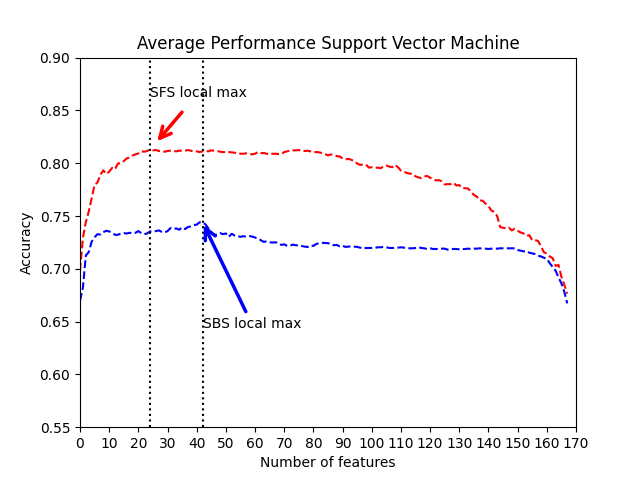
\includegraphics[scale=0.8]{./figures/Figure_3.png}
    \caption{Difference in performance for the SVM classifier}
    \label{fig:svm}
  \end{center}
\end{figure}

Figure \ref{fig:svm} shows that they are a significant difference between the two selection methods for the SVM. The SFS method achieved an accuracy of over 80\% while the SBS method never achieved an accuracy of over 75\%. Furthermore, the SFS method used less features than the SBS method.

\chapter{Discussion}

As mentioned in the result section, the morphological features were overrepresented in terms of being included in the optimal set. Similar results were achieved by DE DÄR ANDRA GRABBARNA ET AL % Refererar vi till dem i Similar works?
who compared deep features generated by a convoluted neural network against SIFT descriptors. They obtained the highest accuracy using only deep featuers. While mixing deep and SIFT features, the accuracy was decreased. Finally only using SIFT features resulted in the worst observed performance. 

% Feature 151
As mentioned in the results, the most prominent feature was feature 151, which is a morphological feature. The feature measures the extent of the lesion, i.e. how many of the pixels in the image are within the lesion. This might be due to the way the tests were conducted. In the forward selection, if a feature is selected early, then it is likely to be contained in the optimal set. Thus the fact that the feature was so common might be an indicator that it was chosen early in the process. Which in turn indicates that the feature is a strong indicator on its own. However, the feature was common in both SBS and SFS, thus it might simply be an effective indicator of malignant melanoma.

% Feature 160
The second most prominent feature was feature 160, which is a color feature. As stated in the results, the feature measures the quotient of the average amount of red color within the lesion over the amount of red color in the surrounding skin. Thus, a high or low value indicates a contrast in terms of red colors between the lesion and the surrounding skin. The prominence of this feature might indicate that a contrast in terms of red color between the surrounding skin and the lesion is a common indicator of malignant melanoma. % Stödjer några källor att just färgen röd är viktigare än blå och grön?

% De stora skillnaderna mellan selection metoder
An interesting result was the difference between the two selection methods for the SVM and KNN classifiers. In both cases the SFS method achieved higher maximum accuracies while at the same time using more features than the SBS. Furthermore, the results  show that during the selection process, the SFS method had a higher average accuracy than the SBS when they utilized the same number of features. They do however converge toward the same accuracy in the beginning and end of the selection process. This indicates that there might be some hidden synergies between features where some combinations give rise to higher performance. Furthermore, this can be an indicator of that it is easier for the selection method to find these synergies when adding features rather than removing them.

Neural network and Random forest did not show any significant difference between the two selection methods. They also used more features on average in their most optimal set. Furthermore, these two models gained less in terms of performance compared to the SVM and KNN classifiers. Hence, the selection models seem to have difficulties to find effective features compared to the other classifiers.

% Att graferna och tabellerna skiljer sig åt

Furthermore, the graphs depicting the average performance of the selection methods for every classifier, and the tables presenting the average number of features used to obtain the highest accuracy for every selection method for every classifier, does not match in terms of the number of features used to obtain the highest accuracy. % Den här meningen är lite konstig. Kanske skriva om den.
For example, in the case of the SVM classifier, the SFS used on average 32,6 features and the SBS 25,4 features to obtain the highest accuracy. Meanwhile, the graph shows that the SFS obtained the highest accuracy around 24 features and the SBS around 42 features. This difference  is most likely due to the method for obtaining the results. In the former case, the accuracy of every iteration of every test was recorded. The average accuracy for every iteration was then calculated, and the graph was plotted. In the latter case, the maximum accuracy and which features constituted the optimal set was recorded. The features were then counted and the average number of features used could hence be calculated. The difference between the two test might be reduced if the number of tests performed was increased. 

% Man kan egentligen stanna tidigare än max max accuracy
Lastly, the graphs  show that for all of the methods, there is an early gain in terms of accuracy which then plateaus to then steadily decline when more and more features are added. The maximum accuracy is usually obtained towards the end of this plateau which results in a marginal gain in accuracy but a vast increase of features which increases the runtime of the algorithms. This is especially true for the KNN classifier using the SFS method, where the accuracy plateaus at around 15 features but the maximum is achieved at around 65 features. There might therefore be an interest in instead of solely measuring the accuracy, to instead introduce a two-factor system where the selection method also takes into account the increase of the feature space. Thus, the method can balance the optimal number of features dependent on both performance and runtime.


\chapter{Conclusions}

From the results, we can say that morphological features are more important than SIFT features for our classifiers' accuracy. However, there is a variance inside the morphological feature set and the best accuracy were achieved with a combination of morphological and SIFT features.

There was some variance between the difference models regarding which features were the most important. The main difference between the models were how many features were used. The SVM and KNN classifiers used fewer features than the NN and RF classifiers. 

Furthermore, the results show that the SFS method is more effective than the SBS method for the SVM and KNN classifiers. However, for the RF and NN classifiers, the two methods were equally effective.

SBS used fewer features for all models except NN, but SFS achieved better accuracy when using as many features as the SBS. % Lite märkligt men vill säga att SFS är bättre än SBS även när SBS är som bäst.

% Print the bibliography (and make it appear in the table of contents)
\printbibliography[heading=bibintoc]

\appendix

\chapter{Something Extra}

% Tailmatter inserts the back cover page (if enabled)
\tailmatter

\end{document}
